\documentclass[12pt]{article}
%% arXiv paper template by Flip Tanedo
%% last updated: Dec 2016



%%%%%%%%%%%%%%%%%%%%%%%%%%%%%
%%%  THE USUAL PACKAGES  %%%%
%%%%%%%%%%%%%%%%%%%%%%%%%%%%%

\usepackage{amsmath}
\usepackage{amssymb}
\usepackage{amsfonts}
\usepackage{graphicx}
\usepackage{xcolor}
\usepackage{nopageno}
\usepackage{enumerate}
\usepackage{parskip}
\usepackage{framed}
%\usepackage{bbm} 
\usepackage[normalem]{ulem}


\renewcommand{\thesection}{}
\renewcommand{\thesubsection}{\arabic{subsection}}

%%%%%%%%%%%%%%%%%%%%%%%%%%%%%%%%%%%%%%%%%%%%%%%
%%%  PAGE FORMATTING and (RE)NEW COMMANDS  %%%%
%%%%%%%%%%%%%%%%%%%%%%%%%%%%%%%%%%%%%%%%%%%%%%%

\usepackage[margin=2cm]{geometry}   % reasonable margins

\graphicspath{{figures/}}	        % set directory for figures

% for capitalized things
\newcommand{\acro}[1]{\textsc{\MakeLowercase{#1}}}    

%\numberwithin{equation}{section}    % set equation numbering
\renewcommand{\tilde}{\widetilde}   % tilde over characters
%\renewcommand{\vec}[1]{\mathbf{#1}} % vectors are boldface

\newcommand{\dbar}{d\mkern-6mu\mathchar'26}    % for d/2pi
\newcommand{\ket}[1]{\left|#1\right\rangle}    % <#1|
\newcommand{\bra}[1]{\left\langle#1\right|}    % |#1>
\newcommand{\Xmark}{\text{\sffamily X}}        % cross out

\let\olditemize\itemize
\renewcommand{\itemize}{
  \olditemize
  \setlength{\itemsep}{1pt}
  \setlength{\parskip}{0pt}
  \setlength{\parsep}{0pt}
}


% Commands for temporary comments
\newcommand{\comment}[2]{\textcolor{red}{[\textbf{#1} #2]}}
\newcommand{\flip}[1]{{\color{red} [\textbf{Flip}: {#1}]}}
\newcommand{\email}[1]{\texttt{\href{mailto:#1}{#1}}}

\newenvironment{institutions}[1][2em]{\begin{list}{}{\setlength\leftmargin{#1}\setlength\rightmargin{#1}}\item[]}{\end{list}}


\usepackage{fancyhdr}		% to put preprint number



% Commands for listings package
%\usepackage{listings}      % \begin{lstlisting}, for code
%
% \lstset{basicstyle=\ttfamily\footnotesize,breaklines=true}
%    sets style to small true-type



%%%%%%%%%%%%%%%%%%%
%%%  HYPERREF  %%%%
%%%%%%%%%%%%%%%%%%%

%% This package has to be at the end; can lead to conflicts
\usepackage{microtype}
\usepackage[
	colorlinks=true,
	citecolor=black,
	linkcolor=black,
	urlcolor=green!50!black,
	hypertexnames=false]{hyperref}





\begin{document}


\begin{center}

    {\Large \textsc{Long HW 7}:
    \textbf{Fermions and Mass}}
    
\end{center}

\vskip .4cm

\noindent
\begin{tabular*}{\textwidth}{rl}
	\textsc{Course:}& Physics 165, \emph{Introduction to Particle Physics} (2018)
	\\
	\textsc{Instructor:}& Prof. Flip Tanedo (\email{flip.tanedo@ucr.edu})
	\\
	\textsc{Due by:}& \textbf{Tuesday}, February 27 
\end{tabular*}

\noindent
This is the main weekly homework set. Unless otherwise stated, give all responses in natural units where $c = \hbar = 1$ and energy is measured in electron volts (usually MeV or GeV). 



\subsection{Follow the spin indices}

In class we argued that a Feynman diagram is shorthand for what amounts to matrix multiplication. 

Consider a theory the theory that we once called QED$+\mu$. The Lagrangian for this theory is:
\begin{align}
	\mathcal L 
	& = 
	\bar \Psi_{(e)} 
	i \gamma^\mu 
	D_\mu
%	\left(\partial_\mu - i e A_\mu\right) 
	\Psi_{(e)}
	+
	\bar \Psi_{(\mu)} 
	i \gamma^\mu 
%	\left(\partial_\mu - i e A_\mu\right)
	D_\mu
	\Psi_{(\mu)} - \frac 14 F_{\mu\nu}F^{\mu\nu}
	- m_{(e)} \bar \Psi_{(e)}\Psi_{(e)}
	- m_{(\mu)} \bar \Psi_{(\mu)}
	\Psi_{(\mu)}
	\ ,
\end{align}
where $D_\mu$ is the \textbf{covariant derivative} that includes the photon field,
\begin{align}
	D_\mu = \partial_\mu - i e A_\mu(x) \ .
\end{align}
$\psi_{(e)}$ and $\psi_{(\mu)}$ are the electron and muon fields respectively. You should recognize the electric gauge coupling ($e$), the electron and muon masses ($m_{(e)}$ and $m_{(\mu)}$). The field strength term $\frac 14 F_{\mu\nu}F^{\mu\nu}$ is the kinetic term for the photon. 

Consider the following Feynman diagram for $e^-e^+ \to \mu^-\mu^+$. 
\begin{center}
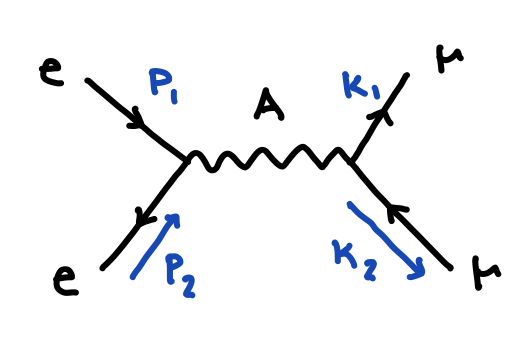
\includegraphics[width=.4\textwidth]{HW7b.png}	
\end{center}
We have drawn the fermion lines with \textbf{Dirac} arrows so that they follow the direction of charge. Recall that the Dirac spinor has the following four components:
\begin{align}
	\Psi =
	\begin{pmatrix}
	\psi_L^\alpha
	\\
	\psi_R^{\dot\alpha}
	\end{pmatrix}
	=
	 \begin{pmatrix}
		\psi_L^\uparrow \\
		\psi_L^\downarrow \\
		\psi_R^\uparrow \\
		\psi_R^\downarrow
	\end{pmatrix}
	=
	\begin{pmatrix}
		\text{left chiral, spin `up'} \\
		\text{left chiral, spin `down'} \\
		\text{right chiral, spin `up'} \\
		\text{right chiral, spin `down'}
	\end{pmatrix} \ .
\end{align}
Here `up' and `down' are relative to the fermion 3-momentum which serves as a quantization axis. The Feynman rules for this theory are:
\begin{center}
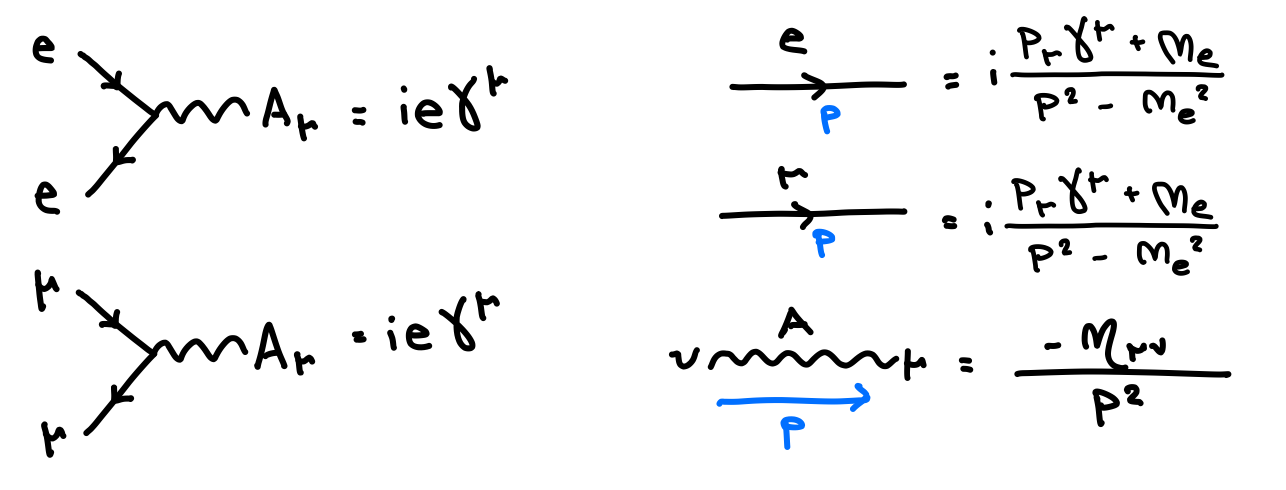
\includegraphics[width=.7\textwidth]{HW7bb.png}	
\end{center}
The $\gamma$ matrices are:
\begin{align}
	\gamma^0 &= 
	\begin{pmatrix}
		0 & 1_{2\times 2} \\
		1_{2\times 2} & 0 
	\end{pmatrix}
	&
	\gamma^i &= 
	\begin{pmatrix}
		0 & \sigma^i \\
		-\sigma^i & 0 
	\end{pmatrix} \ ,
\end{align}
where the $0$'s are $2\times 2$ matrices and $1_{2\times 2}$ is the $2\times 2$ identity matrix. The amplitude for $e^-e^+ \to \mu^-\mu^+$ is a matrix multiplication\footnote{I'm dropping factors of $i$ that are irrelevant for us.}:
\begin{align}
	\mathcal M &=
	e^2\left[ \bar\Psi_{(e)}\gamma^\mu \Psi_{(e)} \right]
	\frac{-\eta_{\mu\nu}}{(p_1+p_2)^2}
	\left[ \bar\Psi_{(\mu)}\gamma^\nu \Psi_{(\mu)} \right]
\end{align}
Here $\bar\Psi = \Psi^\dag \gamma^0$.  The terms in square brackets are matrix multiplications with respect to the spinor indices. Answer the following questions:
\begin{enumerate}
	\item[(a)] Is this process possible when the initial states are a \emph{spin-up, left-handed electron} and a \emph{spin-up, right-handed positron}? (`Possible' means that there's a non-zero amplitude.)
	\item[(b)] Suppose that we fix the vector index $\mu = \nu = 3$ so that we're only looking at one term in the sum over these indices. For this term, is it possible for the initial state to have a \emph{spin-up, left-handed electron}  \emph{spin-up, left-handed positron}?
	\item[(c)] Suppose that we fix the vector index $\mu = \nu = 1$ so that we're only looking at one term in the sum over these indices. For this term, is it possible for the initial state to have a \emph{spin-up, left-handed electron}  \emph{spin-up, left-handed positron}?
	\item[(d)] Suppose that we fix the vector index $\mu = \nu = 2$ so that we're only looking at one term in the sum over these indices. For this term, is it possible for the final state to have a \emph{spin-up, left-handed muon}  \emph{spin-up, left-handed anti-muon}?
	\item[(e)] Is it possible to have the following combination: a \emph{spin-up, left-handed electron} annihilates with a \emph{spin-up, left-handed positron}, turns into an intermediate virtual photon, which then goes to a \emph{spin-up, left-handed muon} and a \emph{spin-down, left-handed anti-muon}? 
\end{enumerate}
If a process is not possible, explain why.


\subsection{Gauge Boson Masses}
The Higgs kinetic term is:
\begin{align}
	\mathcal L_\text{kin}[H] &= |DH|^2 = \left[\left(D_\mu H\right)^\dag\right]_a
		\left(D^\mu H\right)^a
	&
	\left(D_\mu\right)^a_{\phantom{a}b} &= \partial_\mu 
	- i g W^A \left(T^{A}\right)^a_{\phantom{a}b}
	- ig' q_H B_\mu \ .	
\end{align}
Terms with no $a/b$ indices have an implicit $\delta^a_b$. The Higgs hypercharge is $q_H = 1/2$. The $T^A$ are simply the Pauli matrices up to a factor of two:
\begin{align}
	T^1 &= \frac{1}{2}
	\begin{pmatrix}
	0 & 1 \\
	1 & 0	
	\end{pmatrix}
	&
	T^2 &= \frac{1}{2}
	\begin{pmatrix}
	0 & -i \\
	i & 0	
	\end{pmatrix}
	&
	T^3 &= \frac{1}{2}
	\begin{pmatrix}
	1 & 0 \\
	0 & -1	
	\end{pmatrix}
	\ .
\end{align}
Replace $H(x)$ by its constant vacuum expectation value,
\begin{align}
H(x)^a \to H_0^a = 
\frac{1}{\sqrt{2}}
\begin{pmatrix}
	0\\
	v
\end{pmatrix} \ .
\label{eq:Higgs:vev}
\end{align}
Because this is constant, all partial derivatives vanish: $\partial_\mu H_0 = 0$. Show that the remaining terms in $\mathcal L_\text{kin}[H_0]$ can be written in the following form:
\begin{align}
	\mathcal L_\text{kin}[H_0]
	= M_W^2 W_\mu^+ W^{-\mu} + 
	\begin{pmatrix}
		B_\mu & W^3_\mu
	\end{pmatrix}
	\begin{pmatrix}
		M_{11} & M_{12}
		\\
		M_{12} & M_{22}
	\end{pmatrix}
	\begin{pmatrix}
		B^\mu \\ W^{3\mu}
	\end{pmatrix} \ .
	\label{eq:Gauge:mass}
\end{align}
What are the values of $M_W$, $M_{11}$, $M_{12}$, and $M_{22}$ in terms of $g$, $g'$, $q_H$, and $v$.  

\textsc{Hint}: Use the following basis:
\begin{align}
	T^+ &= 
	\begin{pmatrix}
	0 & 1 \\
	0 & 0	
	\end{pmatrix}
	&
	T^- &=
	\begin{pmatrix}
	0 & 0 \\
	1 & 0	
	\end{pmatrix}
	&
	W^\pm = \frac{1}{\sqrt{2}}\left(W^1 \mp i W^2\right) \ .
\end{align}
So that the covariant derivative is
\begin{align}
	\left(D_\mu\right)^a_{\phantom{a}b} &= \partial_\mu 
	- i g W_\mu^+ T^+
	- i g W_\mu^- T^-
	- i g W_\mu^3 T^3
	- ig' q_H B_\mu \ .
\end{align}
Start by calculating $D_\mu H_0$.


\subsection{Yukawa terms}

An additional term that we can throw into the `interactions' part of the Lagrangian takes the following form:
\begin{align}
	\mathcal L_\text{Yuk} &=
	y H^\dag L \bar E + \text{h.c.}
\end{align}
Recall that 
\begin{align}
	L &= \begin{pmatrix}
		\nu_e \\
		e_L
	\end{pmatrix}
	&
	\bar E = e_R^\dag \ .
\end{align}
The coupling constant $y$ is called the \textbf{Yukawa coupling}. If we replace the Higgs field by its vacuum expectation value, $H\to H_0$ in (\ref{eq:Higgs:vev}), what is the electron mass in terms of $v$ and $y$?


\appendix
\vspace{1em}
{\Large\textbf{Extra Credit}}






\subsection{Weyl Arrows}

Draw the diagram in Problem 1 with Weyl fermion arrows.  You should consider all of the possibilities for different chirality combinations of the initial and final state particles. Some combinations are forbidden, you can use indices to figure out which. Recall that $\psi_L^\alpha$ has a left-handed index while $\psi_R^{\dot\alpha}$ has a right-handed index. 

\subsection{Diagonalize the mass matrix}
In (\ref{eq:Gauge:mass}) you derived a mass matrix for the $B$ and $W^3$ bosons. It is not diagonal. Derive the `weak mixing angle' that diagonalizes these into the photon and $Z$ boson:
\begin{align}
	\begin{pmatrix}
		A \\
		Z
	\end{pmatrix}
	=
	\begin{pmatrix}
		\cos\theta_w & \sin\theta_w\\
		-\sin\theta_w & \cos\theta_w
	\end{pmatrix}
	\begin{pmatrix}
		B \\
		W^3
	\end{pmatrix} \ .
\end{align}
Write $\theta_w$ in terms of $g$, $g'$, $q_H$, $v$ and an appropriate inverse trigonometric function.


\subsection{Reading}

Read Richard Slansky's \emph{Lecture Notes: from simple field theories to the standard model} in the \textit{Particle Physics: A Los Alamos Primer} collection\footnote{Link on our course website.}. Explicitly derive (68). In Slansky's notation, $\rho$ is `the' Higgs boson. Comment on:
\begin{itemize}
\item[(a)] The relation between the mass of a spin-1 particle and the coupling to a single Higgs boson.
\item[(b)] The relation between the mass of a spin-1 particle and the coupling to two Higgs bosons.
\item[(c)] Based on this problem and on Problem 3, comment on the relation between the mass of a spin-1/2 particle in the Standard Model and the coupling of that particle to the Higgs boson?
\end{itemize}



\end{document}